\section{1. Medici\'on de distorsi\'on arm\'onica}
El objetivo de esta secci\'on es realizar la medici\'on de la distorsi\'on arm\'onica total de los generadores de funciones
disponibles, para lo cual ser\'a necesario generar una se\~nal senoidal de $f = 800kHz$ con $350mVpp$ de amplitud, y utilizando el
analizador de espectro, observar el contenido espectral de la onda generada y obtener a partir de ello la magnitud de las componentes
espectrales. 

Esto \'ultima, implica hacer el c\'alculo de la Ec. \ref{eq:THD_theory}. Donde la potencia de los arm\'onicos se mide directamente
en unidades de dBm, y se obtiene la potencia correspondiente a cada arm\'onico.

\begin{equation}
    THD = \frac{ \sum_{i = 1}^{n} P_i }{P_0}
    \label{eq:THD_theory}
\end{equation}

% Subdividir las subsecciones por cada tipo de generador utilizado
% recordando poner las mediciones completas, el resultado numerico y luego
% el error. Contrastando con las especificaciones de la hoja de datos.

\subsection{Mediciones}
En las Figs. \ref{fig:thd_agilent}, \ref{fig:thd_gwinstek} y \ref{fig:thd_picotest} se pueden observar
las mediciones realizadas para el espectro de la onda senoidal antes descripta, en los casos de tres marcas de generadores senoidales,
de forma tal que luego utilizando la opci\'on Marker del analizador de espectro, se obtienen mediciones de cada uno de los arm\'onicos
en una cantidad finita hasta que la amplitud o magnitud no produce cambio apreciable en el valor de THD, o no se miden m\'as arm\'onicos.

\begin{figure}[H]
    \centering
    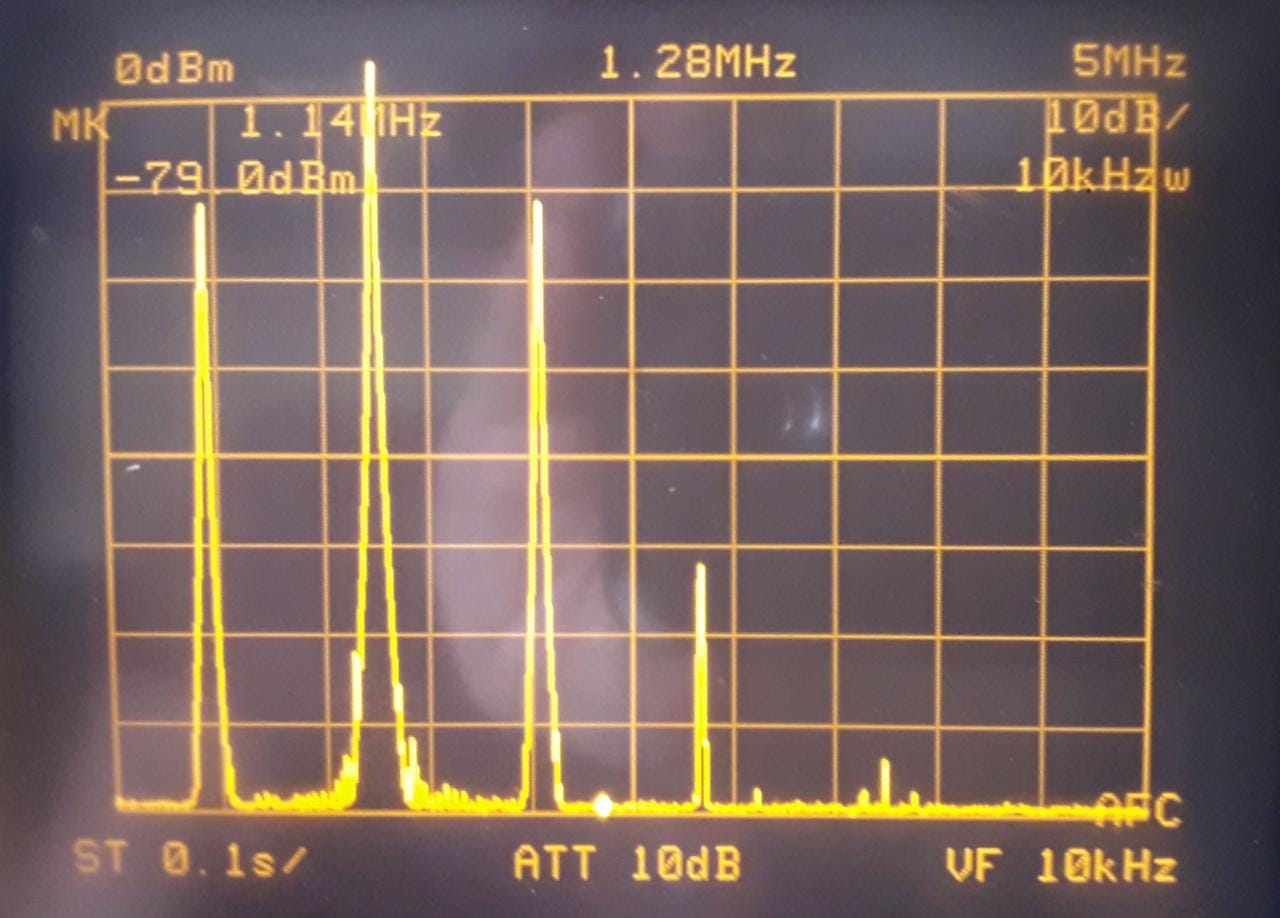
\includegraphics[scale=0.2]{../Mediciones/Ejercicio_1/generador_agilent.jpeg}
    \caption{Espectro de onda senoidal de generador Agilent}
    \label{fig:thd_agilent}
\end{figure}

\begin{figure}[H]
    \centering
    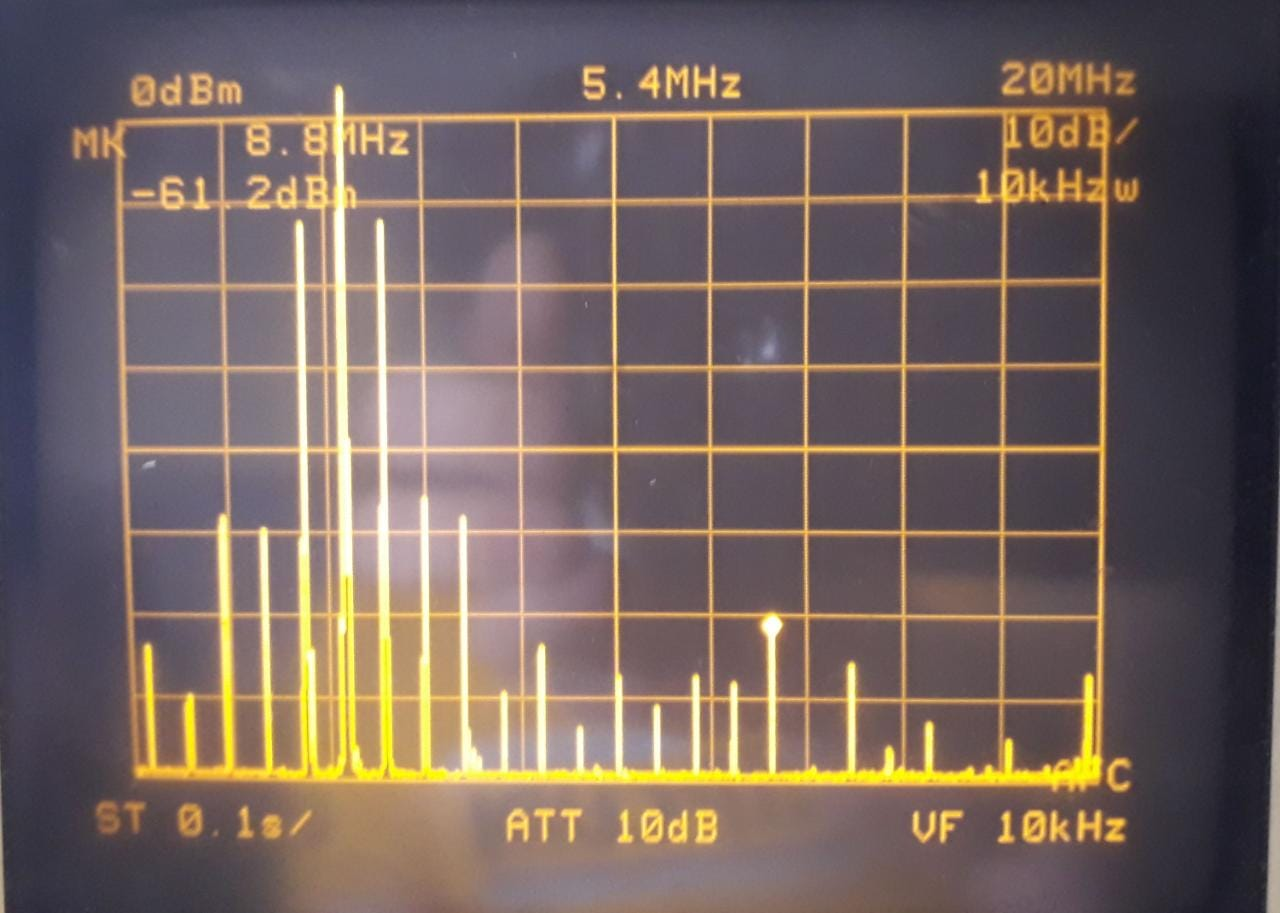
\includegraphics[scale=0.2]{../Mediciones/Ejercicio_1/generador_gwinstek.jpeg}
    \caption{Espectro de onda senoidal de generador GW Instek}
    \label{fig:thd_gwinstek}
\end{figure}

\begin{figure}[H]
    \centering
    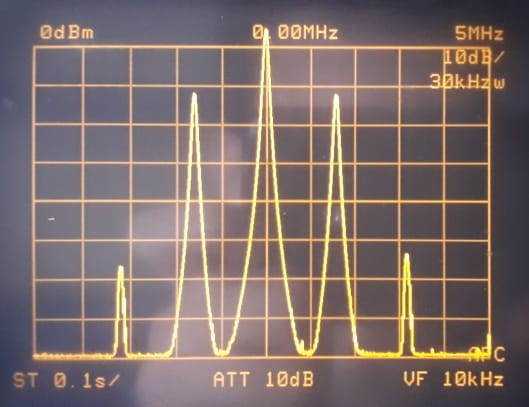
\includegraphics[scale=0.65]{../Mediciones/Ejercicio_1/generador_picotest.jpeg}
    \caption{Espectro de onda senoidal de generador Picotest}
    \label{fig:thd_picotest}
\end{figure}

\begin{table}[H]
    \centering
    \begin{tabular}{c c c}
        Fundamental [dBm] & Primer arm\'onico [dBm] & $THD_P$ [$\%$]\\
        \hline \\
        $-11$ & $-51.8$ & $0.0083\%$ \\
        \hline
    \end{tabular}
    \caption{THD del generador Agilent}
\end{table}

\begin{table}[H]
    \centering
    \begin{tabular}{c c c c c c c c c c c}
        $f_o$ & $1^{\circ}$ & $2^{\circ}$ & $3^{\circ}$ & $4^{\circ}$ & $5^{\circ}$ & $6^{\circ}$ & $7^{\circ}$ & $8^{\circ}$ & $9^{\circ}$ & $THD_P$ [$\%$] \\
        \hline \\
        $-12$ & $-45.2$ & $-47.2$ & $-70$ & $-62.6$ & $-77$ & $-65.8$ & $-79.4$ & $-67.2$ & $-61$ & $0.081 \%$ \\
        \hline
    \end{tabular}
    \caption{THD del generador GW Instek, mediciones en dBm}
\end{table}

\begin{table}[H]
    \centering
    \begin{tabular}{c c c}
        Fundamental [dBm] & Primer arm\'onico [dBm] & $THD_P$ [$\%$]\\
        \hline \\
        $-11.8$ & $-53.4$ & $0.0069\%$\\
        \hline
    \end{tabular}
    \caption{THD del generador Picotest}
\end{table}

\subsection{An\'alisis de resultados}
En los resultados obtenidos de las mediciones de THD para cada uno de los generadores, en primer lugar
se puede realizar una comparaci\'on que denota la calidad de tales instrumentos o equipos. En primer lugar,
tanto el Picotest como el Agilent tienen una distorsi\'on arm\'onica baja, al punto en que s\'olo es apreciable en baja
magnitud el primer arm\'onico siguiente al fundamental. Por otro lado, el generador GW Instek posee una gran cantidad de arm\'onicos
y con ello un distorsi\'on arm\'onica casi 10 veces mayor que los otros.

Los resultados obtenidos para el THD calculado en funci\'on de las potencias, dan valores que se encuentren por debajo de los establecido por la hoja de datos en tres \'ordenes de magnitud,
por ello se lleg\'o a la conclusi\'on de que los valores dados por el fabricante est\'an calculados en funci\'on del valor RMS de los arm\'onicos.
Seg\'un los fabricantes, el THD del Agilent deber\'ia estar en torno al $0.04\%$, el del GW Instek en torno al $1 \%$ y para el Picotest debajo de $0.06\%$.
Se atribuyen las diferencias entre las hojas de datos de los fabricantes y los resultados obtenidos, al uso diario y el tiempo de vida que llevan
estos equipos.


\subsection{Conclusiones}
Se pudo observar que en relaci\'on, la distorsi\'on arm\'onica del GW Instek es peor que la del Picotest, y la de este es peor que la del Agilent, seg\'un cada fabricante. Esta es una de las razones,
por las cuales se pueden observar diferencias de precios entre tales marcas.